\documentclass[a4paper]{elektr}
\usepackage{fontspec}
\setmainfont{Times.TTF}[Path=fonts/,BoldFont=Timesbd.TTF,ItalicFont=Timesi.TTF,BoldItalicFont=Timesbi.TTF]
\usepackage{amsmath,amssymb,graphicx,booktabs,array,tabularx,placeins}
\usepackage{hyperref}
\hypersetup{colorlinks=true,allcolors=black,pdftitle={Facial regions and late fusion for deepfake detection}}

\emergencystretch=1em
\renewcommand{\topfraction}{0.95}\renewcommand{\bottomfraction}{0.9}\renewcommand{\textfraction}{0.05}\renewcommand{\floatpagefraction}{0.7}
\setlength{\paperwidth}{210mm}\setlength{\paperheight}{297mm}\setlength{\tabcolsep}{4pt}
\renewcommand{\figurename}{Figure}
\renewcommand{\tablename}{Table}
\renewcommand{\refname}{References}
\renewcommand{\abstractname}{Abstract}
\renewenvironment{abstract}{\par\vskip 1em\small\noindent\textbf{Abstract:}\ }{\par}
\yil{}\vol{}\fpage{}\lpage{}\doi{}
\title{Comparison of eyebrow, eye, and mouth regions for deepfake detection and late fusion analysis}
\author[]{\textbf{Kader TERİK, Nazlıcan AYDEMİR, Dilara ÖZTÜRK,}\\[0.3em]\textbf{Mustafa Furkan CEYLAN, Özge ÇELİK}}
\makeatletter
\gdef\@surnames{Turk J Elec Eng \& Comp Sci}
\def\serieslogo@{\hfill\small\normalfont Turk J Elec Eng \& Comp Sci}
\def\@maketitle{\newpage\null\vskip 4em\begin{center}
{\large\bfseries\@title\par}\vskip 1em
{\small\begin{tabular}{c}\@author\end{tabular}\par}
\vskip 0.8em\end{center}}
\makeatother
\begin{document}
\maketitle

\begingroup
\begin{abstract}
This study examines the discriminative contribution of anatomical facial regions to deepfake detection and whether combining these regions provides additional performance gains. Eyebrow, eye, and mouth regions of interest were evaluated using Xception, EfficientNet-B0, Swin V2 Tiny, and Swin V2 Tiny + Texture on a pool of 3,000 source frames, comprising 1,500 real and 1,500 fake frames, compiled from the FaceForensics project distribution. Full-test ROC-AUC (area under the receiver operating characteristic curve) followed a mouth--eye--eyebrow ordering in all four configurations; Swin V2 Tiny achieved a mouth ROC-AUC of 0.8607. The same ordering was observed in a common test cohort of 196 samples with all three regional scores available. Equal and validation-weighted late fusion were compared on this cohort. Weighted fusion yielded higher ROC-AUC point estimates than equal fusion for all four configurations but did not exceed mouth-only performance. For Swin V2 Tiny, mouth-only and weighted-fusion ROC-AUC values on the common cohort were 0.8803 and 0.8763, respectively. In a paired bootstrap analysis with 5,000 resamples, the 95\% confidence intervals for all eight fusion-minus-mouth AUC differences included zero. Decision-change analysis showed that fusion corrected some mouth errors while overturning some correct mouth decisions. The study compares three anatomical regions and two fusion rules under a controlled experimental protocol rather than proposing a new architecture. The findings are limited to the present data and protocol; no additional ROC-AUC gain from multi-region fusion was demonstrated.

\keywords{Anatomical feature analysis, deepfake detection, error overlap, score aggregation, visual classification}
\end{abstract}
\endgroup

\section{Introduction and related work}
Realistic facial manipulations raise concerns about the reliability of digital content and increase the need for automated verification. FaceForensics++ is widely used to evaluate detection methods in this field \cite{rossler}. The regional analysis by Tolosana et al. shows that the discriminative strength of facial regions depends on the dataset and evaluation conditions \cite{tolosana}. High performance in a particular region therefore cannot be assumed to generalize automatically to other manipulations or datasets.

Convolutional neural networks (CNNs) learn local image patterns, while attention mechanisms emphasize informative areas \cite{zhao}. Xception uses depthwise separable convolutions, and EfficientNet uses compound scaling \cite{chollet,tan}. Swin Transformer V2 constructs hierarchical representations through shifted-window self-attention \cite{swin}. This study evaluates two CNNs, a Transformer, and a hybrid configuration combining Transformer features with texture descriptors. Because training settings differ across model families, the comparison does not isolate architectural effects under an equal computational budget.

Studies focusing on anatomical regions exploit different types of information. Eye-blink methods use physiological and temporal behavior \cite{li,jung}, whereas LipForensics and DFT-MF examine mouth motion \cite{haliassos,elhassan}. The eyebrow biometrics approach of Nguyen and Derakhshani relies on identity-based matching \cite{nguyen}. Here, static eyebrow, eye, and mouth regions of interest (ROIs) are used as inputs for binary classification; this task is not directly equivalent to temporal or identity-based detection.

Recent studies investigate different forms of local representation and fusion. Soudy et al. (2024) combined regional decisions from CNN and convolutional vision Transformer models through majority voting \cite{soudy}. Mirzayev and Dibeklioğlu (2024) addressed spatiotemporal inconsistencies using learnable feature operations inspired by motion magnification networks, without directly applying motion magnification \cite{mirzayev}. Anand et al. (2025) examined localized manipulations using action unit-guided video representations and cross-attention-based representation fusion \cite{anand}. Lei et al. (2025) evaluated facial geometry and texture information within a decision-fusion and adversarial-defense framework \cite{lei}. The hybrid approach of Shivaprakash et al. (2026) combined Swin V2 features with local binary pattern (LBP), gray-level co-occurrence matrix (GLCM), Gabor, and wavelet descriptors \cite{shivaprakash}. These feature- or representation-fusion methods differ from the present late-fusion approach, which combines probabilities from independently trained ROI models.

Karimi and Dibeklioğlu (2024) examined the difficulty of separating spurious and invariant features in domain generalization \cite{karimi}. Their study is not specific to deepfakes; it provides methodological context for the need to test whether performance on one data source transfers to unseen domains. The present experiments do not establish cross-dataset generalization.

The research questions are: (RQ1) How does performance differ among eyebrow, eye, and mouth ROIs under the present protocol? (RQ2) How do the four model configurations perform across these regions? (RQ3) Do equal and validation-weighted late fusion provide additional ROC-AUC over the strongest single region on the same common cohort?

Whereas the reviewed studies consider temporal, biometric, or other fusion approaches, this study compares four model configurations across eyebrow, eye, and mouth ROIs using a common source pool and evaluation protocol. Its contributions also include evaluating equal and validation-weighted late fusion on the same common test cohort and examining single-region versus fusion performance through bootstrap uncertainty and error patterns. No new deep learning architecture or superiority over full-face methods is claimed.

\section{Materials and methods}
The experiment has two evaluation stages: regional evaluation on each ROI's available full test set, followed by paired comparisons on the common cohort with all three ROIs available. Figure~\ref{fig:workflow}(a) shows the experimental workflow, and Figure~\ref{fig:workflow}(b) presents example frames from the test subset.
\begin{figure}[!htbp]\centering\begin{minipage}{15.8cm}
\centering
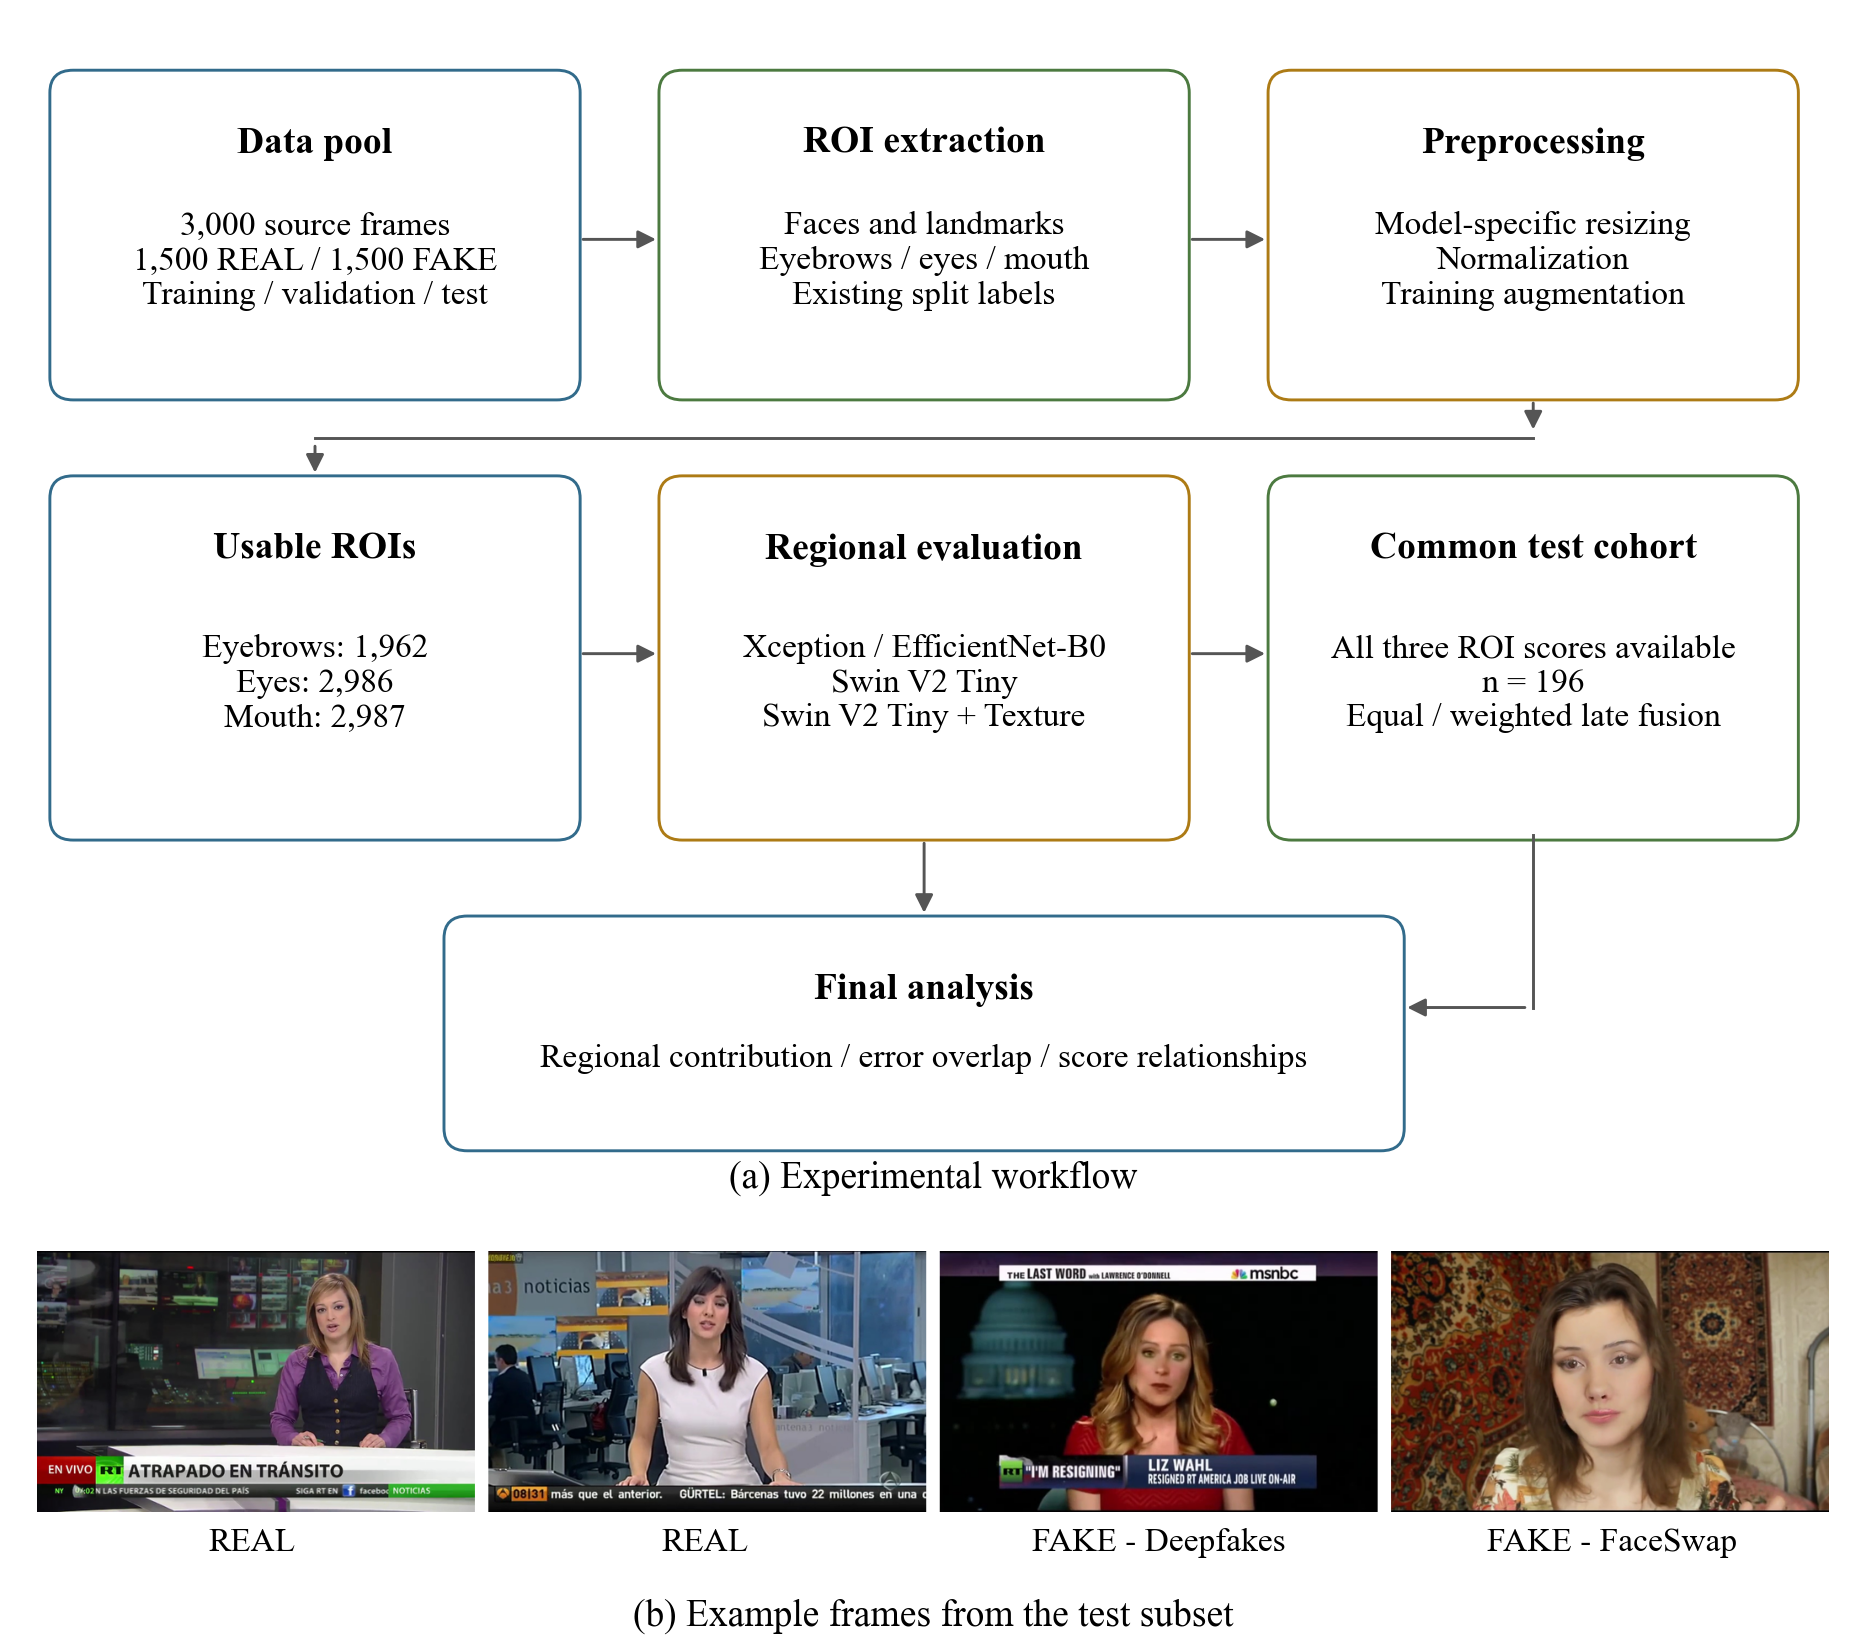
\includegraphics[width=\linewidth]{assets/figure1_complete.png}
\caption{Experimental setup and data examples. (a) Regional evaluation and three-ROI late fusion; (b) from left to right, two REAL examples, one Deepfakes example, and one FaceSwap example.}\label{fig:workflow}
\end{minipage}\end{figure}
The frames in Figure~\ref{fig:workflow}(b) illustrate data diversity only; they were not selected as easy or difficult examples for the models. The source-level split shown in the diagram should be interpreted in light of the metadata checks described below. Because the source pool contains six manipulation labels, its definition is not synonymous with the standard four-method FaceForensics++ subset alone.

\subsection{Data pool and partitioning}
The pool compiled from the FaceForensics project distribution contains 1,500 REAL and 1,500 FAKE source frames. Source frames were divided into training, validation, and test subsets at an 80/10/10 ratio. Table~\ref{tab:data} reports the data composition and ROI distribution.
\begin{table}[!htbp]\centering\begin{minipage}{15.8cm}
\caption{Distribution of source frames and usable ROI records.}\label{tab:data}
\centering \small
\begin{tabular}{lrrrr}\toprule
Source / region & Training & Validation & Test & Total \\\midrule
REAL & 1200 & 150 & 150 & 1500 \\
Deepfakes & 190 & 32 & 31 & 253 \\
Face2Face & 208 & 19 & 24 & 251 \\
FaceSwap & 180 & 22 & 20 & 222 \\
NeuralTextures & 163 & 14 & 20 & 197 \\
FaceShifter & 211 & 35 & 31 & 277 \\
DeepFakeDetection & 248 & 28 & 24 & 300 \\
Total FAKE & 1200 & 150 & 150 & 1500 \\
Total source frames & 2400 & 300 & 300 & 3000 \\
\midrule Eyebrow ROI & 1562 & 204 & 196 & 1962 \\
Eye ROI & 2388 & 296 & 302 & 2986 \\
Mouth ROI & 2389 & 296 & 302 & 2987 \\
\bottomrule\end{tabular}
\par\smallskip\begin{minipage}{\linewidth}\small Source-frame counts and ROI-record counts are different units. The common fusion test cohort comprises 196 source-frame keys: 101 REAL and 95 FAKE.\end{minipage}
\end{minipage}\end{table}

The FAKE class in Table~\ref{tab:data} comprises six manipulation sources. ROI counts differ from source-frame counts because of ROI acceptance conditions and multiple faces. There were 1,962 usable eyebrow records, 2,986 eye records, and 2,987 mouth records. The source-selection metadata reported that original source folders within the same class did not occur in more than one split. This check alone does not establish identity-level separation or separation of all manipulations derived from the same real source video using a common root-video identifier. ROI records retained their existing split labels. Validation data were used for model/checkpoint selection and fusion weights; test data were used only for final evaluation.

\subsection{ROI extraction and preprocessing}
Faces and landmarks were detected using MediaPipe Face Landmarker. The mouth ROI was defined using 40 lip landmarks and a surrounding margin, while the combined eye ROI included both eyes. The eyebrow ROI used 20 landmarks and required a minimum width of 48 pixels, a minimum height of 14 pixels, and an eye-landmark inclusion ratio no greater than 0.25. The minimum-size thresholds excluded very small eyebrow crops, while the eye-landmark threshold limited excessive inclusion of the eye region. These are acceptance thresholds for the experimental pipeline rather than standards established in the literature. Images were resized and normalized according to model requirements, with $224 \times 224$ inputs used in most configurations. Data augmentation was applied only to the training subset.

Each eye and mouth test pipeline produced 310 face records from 300 source frames; faces were not detected in eight records, leaving 302 successful ROIs. The eyebrow pipeline yielded 196 successful records and rejected 104: 82 for insufficient cropping space below the eyebrows, 12 for failure to detect a face, 7 for multiple faces, and 3 for other geometric checks. The stricter eyebrow acceptance conditions limited both training data and the common fusion cohort.

The eye and mouth test metadata contain two successful ROIs for each of 10 frames. In nine frames, the face00 and face01 boxes correspond to different face locations; for \texttt{fake\_test\_00075}, the two records largely overlap on the same foreground face. This frame was not included in the fusion cohort, and the full regional test results were not recomputed after removing these duplicate records. Among frames with multiple ROIs, only \texttt{fake\_test\_00088} entered the common cohort with a successful eyebrow ROI. The face00 eye and mouth scores were used for this frame. All three face00 crops corresponded to the same face of the main presenter. The common cohort was constructed using this single-face selection rule.

\subsection{Model configurations and training}
Xception and EfficientNet-B0 are CNN configurations, whereas Swin V2 Tiny is a Transformer configuration. Swin V2 Tiny + Texture is a hybrid that combines image representations with LBP, GLCM, Gabor, and wavelet texture features. Models were trained with ImageNet-pretrained weights, primarily using Python and Google Colab. Table~\ref{tab:settings}(a) reports the training settings; panels (b) and (c) report the validation-based fusion parameters and regional decision thresholds, respectively.

In the hybrid configuration, the classification head of Swin V2 Tiny was removed to obtain image representations. LBP, GLCM, Gabor, and wavelet features were processed in a separate texture branch using standardization parameters fitted exclusively on the training set. The image and texture branch outputs were each projected to 256-dimensional representations, then concatenated at the feature level into a single 512-dimensional representation. This combined representation was passed to a binary classifier.
\begin{table}[!htbp]\centering\begin{minipage}{15.8cm}
\caption{Training settings, fusion parameters, and regional decision thresholds.}\label{tab:settings}
\centering\small
\textbf{(a) Training settings}\par\smallskip
\begin{tabular*}{\linewidth}{@{\extracolsep{\fill}}lrrrr@{}}\toprule
Model & Batch size & Base LR & Backbone / fine-tuning LR & Weight decay\\\midrule
Xception & 16 & $1\times10^{-4}$ & $1\times10^{-5}$ & Eye: $1\times10^{-4}$\\
EfficientNet-B0 &32&$1\times10^{-3}$&$2\times10^{-5}$&$1\times10^{-4}$\\
Swin V2 Tiny &32&$1\times10^{-4}$&$1\times10^{-5}$&$1\times10^{-2}$\\
Swin V2 Tiny + Texture &16&$2\times10^{-4}$&$2\times10^{-5}$&$1\times10^{-4}$\\\bottomrule
\end{tabular*}
\par\medskip
\textbf{(b) Validation ROC-AUC and fusion weights}\par\smallskip
\begin{tabular*}{\linewidth}{@{\extracolsep{\fill}}lrrrrrr@{}}\toprule
&\multicolumn{3}{c}{Validation ROC-AUC}&\multicolumn{3}{c}{Fusion weights}\\
Model & Eyebrow & Eye & Mouth & $w_{\mathrm{brow}}$ & $w_{\mathrm{eye}}$ & $w_{\mathrm{mouth}}$\\\midrule
Xception&0.6710&0.7252&0.8228&0.2378&0.3132&0.4490\\
EfficientNet-B0&0.6819&0.7129&0.7969&0.2630&0.3078&0.4292\\
Swin V2 Tiny&0.7191&0.8454&0.8858&0.2306&0.3634&0.4060\\
Swin V2 Tiny + Texture&0.7280&0.7222&0.8604&0.2812&0.2742&0.4446\\\bottomrule
\end{tabular*}
\par\medskip
\textbf{(c) Regional decision thresholds}\par\smallskip
\begin{tabular*}{\linewidth}{@{\extracolsep{\fill}}lrrr@{}}\toprule
Model & Eyebrow & Eye & Mouth\\\midrule
Xception & 0.500 & 0.305 & 0.500\\
EfficientNet-B0 & 0.280 & 0.220 & 0.190\\
Swin V2 Tiny & 0.120 & 0.275 & 0.405\\
Swin V2 Tiny + Texture & 0.330 & 0.265 & 0.455\\\bottomrule
\end{tabular*}
\par\smallskip\begin{minipage}{\linewidth}\small
Xception: frozen backbone followed by fine-tuning. EfficientNet-B0: 5 epochs with a frozen backbone and 15 fine-tuning epochs. Swin V2 Tiny: 20 epochs with validation ROC-AUC monitoring; the base LR applies to the classification head. Hybrid: 30 epochs, with backbone unfreezing in later stages. LR denotes learning rate; all models use ImageNet pretraining. Weights are rounded to four decimal places for display. The Xception eyebrow/mouth code does not pass weight decay to Adam; the Xception entry in this column applies only to the eye experiment. Xception eyebrow/mouth thresholds are fixed at 0.50; other regional thresholds are selected using validation F1.
\end{minipage}\end{minipage}\end{table}

No systematic hyperparameter search with equal budgets was performed across model families. Data augmentation and classification-head settings were defined separately for each model configuration. Using the validation data for both checkpoint selection and fusion weights may introduce bias toward the validation set.

\subsection{Common cohort and late fusion}
Regional models were not retrained for fusion. Eyebrow, eye, and mouth FAKE probabilities from the same model family were matched using source-frame keys. An inner join retaining records with all three scores produced 196 records: 101 REAL and 95 FAKE. The common set contains all successful eyebrow test frames; eye-only and mouth-only results were also recomputed on the same keys.

Equal fusion is defined in Eq.~\eqref{eq:equal}, validation contributions and normalized weights in Eq.~\eqref{eq:weights}, and weighted fusion in Eq.~\eqref{eq:weighted}:
\begin{equation}\label{eq:equal}
P_{\mathrm{equal}}=(P_{\mathrm{brow}}+P_{\mathrm{eye}}+P_{\mathrm{mouth}})/3.
\end{equation}
\begin{equation}\label{eq:weights}
r_i=\max(\mathrm{AUC}^{\mathrm{val}}_i-0.5,\epsilon),\qquad
w_i=\frac{r_i}{\sum_jr_j},\qquad i,j\in\{\mathrm{brow,eye,mouth}\}.
\end{equation}
\begin{equation}\label{eq:weighted}
P_{\mathrm{weighted}}=\sum_iw_iP_i,\qquad\sum_iw_i=1.
\end{equation}
$P_i$ is the FAKE probability from the corresponding ROI model, $\mathrm{AUC}^{\mathrm{val}}_i$ is its validation ROC-AUC, and $\epsilon$ is a small positive constant for numerical stability. Weights were determined exclusively from validation data, without using test information. The mouth received the highest weight in all four models. A probability of $P\geq0.50$ was classified as FAKE in common-cohort error and fusion analyses; full regional accuracy/F1 results use the thresholds in Table~\ref{tab:settings}.

\subsection{Metrics, bootstrap, and error analysis}
Regional decision thresholds were not selected from test data. A fixed threshold of 0.50 was used for Xception eyebrow/mouth experiments; the threshold maximizing validation F1 was used for Xception eye, EfficientNet-B0, Swin V2 Tiny, and hybrid experiments. Thresholds were searched in steps of 0.005 over 0.05--0.95 for Xception eye, EfficientNet-B0, and Swin, and over 0.10--0.90 for the hybrid. For EfficientNet-B0, F1 ties were resolved first by higher balanced accuracy, then by proximity to 0.50; the other searches selected the first maximum. The selected threshold was fixed for the corresponding final test. Common-cohort error/fusion comparisons use 0.50 for all regions. The main regional comparison is based on threshold-independent ROC-AUC.

FAKE is the positive class and REAL the negative class. TP/TN denote true positives/negatives, and FP/FN denote false positives/negatives. Accuracy, precision, recall, specificity, F1, and balanced accuracy were calculated using Eq.~\eqref{eq:metrics}:
\begin{equation}\label{eq:metrics}
\begin{aligned}
\mathrm{Accuracy}&=\frac{TP+TN}{TP+TN+FP+FN},&
\mathrm{Precision}&=\frac{TP}{TP+FP},\\
\mathrm{Recall}&=\frac{TP}{TP+FN},&
\mathrm{Specificity}&=\frac{TN}{TN+FP},\\
\mathrm{F1}&=\frac{2TP}{2TP+FP+FN},&
\mathrm{Balanced\ accuracy}&=\frac{\mathrm{Recall}+\mathrm{Specificity}}{2}.
\end{aligned}
\end{equation}
The area under the receiver operating characteristic curve (ROC-AUC) is the primary threshold-independent comparison metric; the area under the precision--recall curve (PR-AUC) summarizes precision--recall performance. Threshold-dependent decision counts and ROC-AUC ranking performance are distinct concepts.

The fusion difference was defined as $\Delta\mathrm{AUC}=\mathrm{AUC}_{\mathrm{fusion}}-\mathrm{AUC}_{\mathrm{mouth}}$. A sample-level paired bootstrap with 5,000 resamples and random seed 42 was applied to the common cohort, using the same indices for mouth and fusion scores in each resample. Single-class resamples were excluded, and 95\% confidence intervals were obtained from the 2.5th and 97.5th percentiles of the distribution. No multiple-comparison correction was applied to the eight comparisons. Sample-level resampling does not model dependence among frames from the same video.

For error analysis, a correct/incorrect decision vector was constructed for each ROI at a threshold of 0.50, and the eight mutually exclusive combinations across the three ROIs were counted. Samples misclassified by the mouth model but correctly classified by fusion were termed ``corrected''; samples correctly classified by the mouth model but misclassified by fusion were termed ``overturned''. The net effect is the number corrected minus the number overturned. Score relationships were examined using Spearman rank correlation; low correlation alone does not establish useful complementarity.

\section{Results}
\subsection{Regional results}
Table~\ref{tab:regional} reports accuracy, F1, and ROC-AUC on the full regional test sets alongside ROC-AUC recomputed on the common cohort. The full eyebrow test set and common cohort each contain 196 samples; the full eye and mouth test sets each contain 302. Differences between full-test and common-cohort values reflect the different sample sets.
\begin{table}[!htbp]\centering\begin{minipage}{15.8cm}
\caption{Regional performance on full test sets and the common cohort.}\label{tab:regional}
\centering \small
\begin{tabular}{llrrrr}\toprule
Model & ROI & Accuracy (\%) & F1 (\%) & Full-test AUC & Common AUC \\\midrule
Xception & Eyebrow & 51.53 & 55.81 & 0.5513 & 0.5513 \\
 & Eye & 57.28 & 70.34 & 0.6770 & 0.6668 \\
 & Mouth & 70.20 & 72.22 & 0.7662 & 0.7527 \\
EfficientNet-B0 & Eyebrow & 54.59 & 65.10 & 0.5874 & 0.5874 \\
 & Eye & 63.58 & 72.08 & 0.7286 & 0.7313 \\
 & Mouth & 71.52 & 76.76 & 0.8332 & 0.8334 \\
Swin V2 Tiny & Eyebrow & 53.57 & 65.92 & 0.6815 & 0.6815 \\
 & Eye & 69.87 & 72.84 & 0.7868 & 0.7829 \\
 & Mouth & 80.46 & 80.91 & 0.8607 & 0.8803 \\
Swin V2 Tiny + Texture & Eyebrow & 60.20 & 67.23 & 0.6688 & 0.6688 \\
 & Eye & 61.26 & 69.77 & 0.7090 & 0.6756 \\
 & Mouth & 71.85 & 74.47 & 0.7918 & 0.7897 \\
\bottomrule\end{tabular}
\par\smallskip\begin{minipage}{\linewidth}\small Full-test sizes: eyebrows 196, eyes and mouth 302. Common cohort: 196 (101 REAL, 95 FAKE). Accuracy/F1 use the regional thresholds in Table~\ref{tab:settings}; common-cohort error/fusion analyses use 0.50. Threshold-dependent metrics are percentages; ROC-AUC is on a 0--1 scale.\end{minipage}
\end{minipage}\end{table}

All four configurations show the mouth $>$ eye $>$ eyebrow ordering of AUC point estimates on both the full test sets and common cohort. Swin V2 Tiny achieved the highest full-test AUC in each region: 0.6815 for eyebrows, 0.7868 for eyes, and 0.8607 for the mouth. EfficientNet-B0 achieved a mouth AUC of 0.8332. The hybrid yielded the highest threshold-dependent eyebrow results, with 60.20\% accuracy and 67.23\% F1, but its AUC remained below the base Swin model in all three ROIs. Accuracy/F1 results obtained under different threshold-selection rules are not evidence of architectural superiority alone; the primary comparison uses ROC-AUC.

Figures~\ref{fig:roc}(a), \ref{fig:roc}(b), and \ref{fig:roc}(c) show the full-test ROC curves for Swin V2 Tiny for mouth, eyes, and eyebrows, respectively. The mouth model has the highest AUC; the AUC ordering does not imply that one ROC curve dominates the others at every threshold.
\begin{figure}[!htbp]\centering\begin{minipage}{15.8cm}\centering
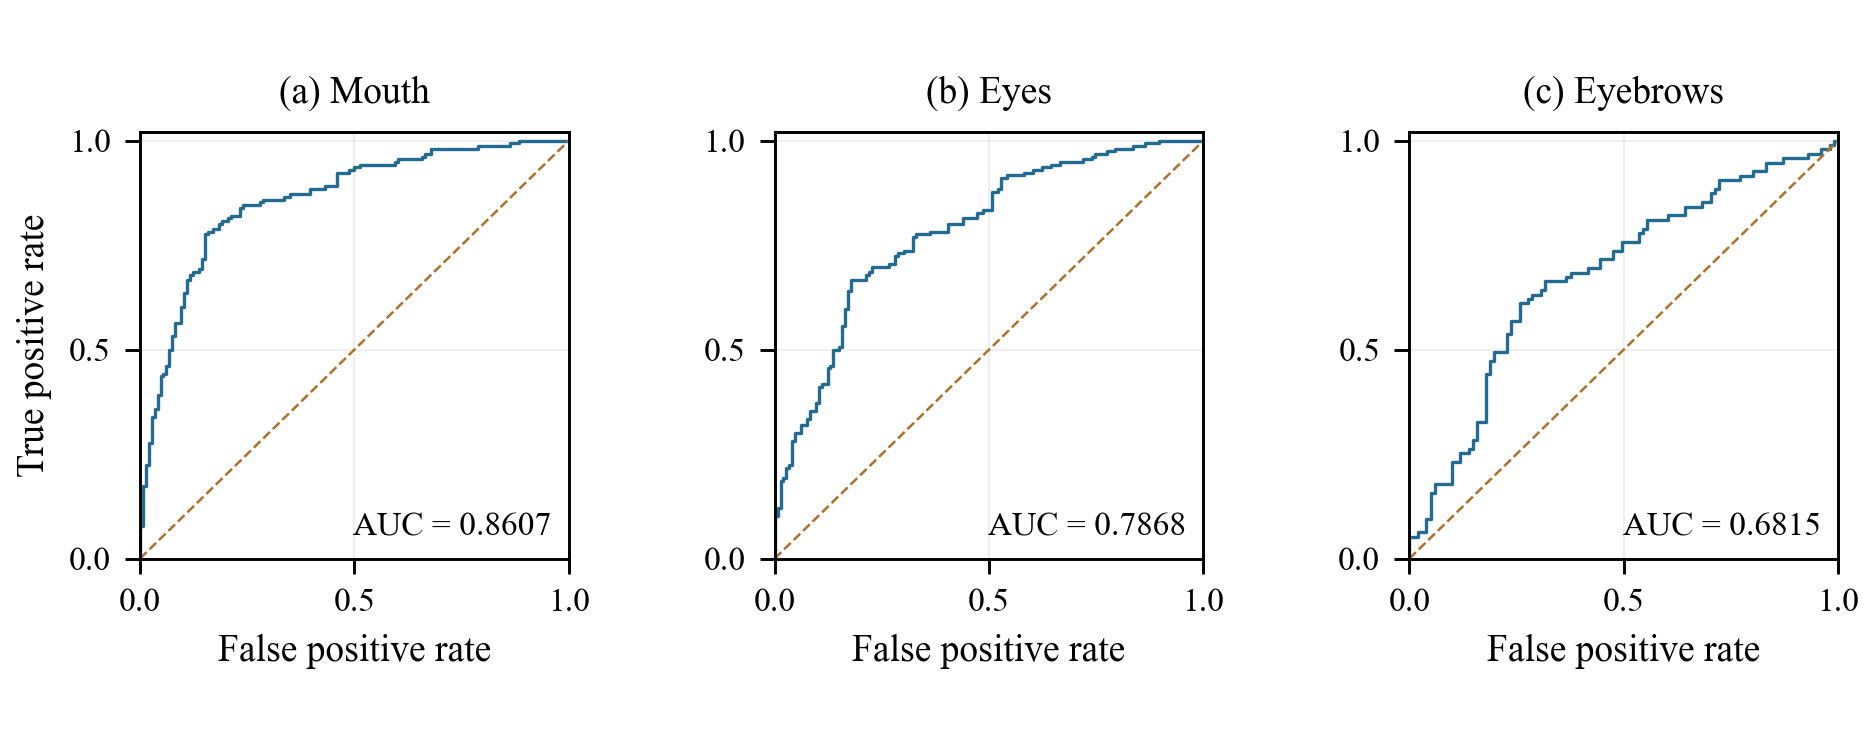
\includegraphics[width=\linewidth]{assets/roc_combined.png}
\caption{Full-test ROC curves for Swin V2 Tiny. (a) Mouth, (b) eyes, (c) eyebrows.}\label{fig:roc}
\end{minipage}\end{figure}

Table~\ref{tab:subgroup} presents an exploratory analysis of Swin V2 Tiny regional AUC by manipulation type. Each FAKE subgroup was compared with the same 101 REAL samples.
\begin{table}[!htbp]\centering\begin{minipage}{15.8cm}
\caption{Exploratory manipulation-subgroup ROC-AUC values for Swin V2 Tiny on the common cohort.}\label{tab:subgroup}
\centering \small
\begin{tabular}{lrrrr}\toprule
Manipulation & FAKE count & Eyebrow AUC & Eye AUC & Mouth AUC \\\midrule
Deepfakes & 21 & 0.6841 & 0.9128 & 0.8689 \\
FaceShifter & 24 & 0.8156 & 0.8412 & 0.9068 \\
NeuralTextures & 13 & 0.5598 & 0.5385 & 0.8576 \\
Face2Face & 17 & 0.6500 & 0.7443 & 0.8567 \\
FaceSwap & 14 & 0.4767 & 0.6690 & 0.8501 \\
DeepFakeDetection & 6 & 0.9670 & 1.0000 & 1.0000 \\
\bottomrule\end{tabular}
\par\smallskip\begin{minipage}{\linewidth}\small Each row uses 101 REAL samples. Because the FAKE subgroups are small, these values do not constitute a confirmatory test of superiority across manipulations.\end{minipage}
\end{minipage}\end{table}

The mouth achieved the highest AUC in four subgroups, while the eye performed better for Deepfakes. Although eye and mouth AUC values for DeepFakeDetection were 1.0000, that subgroup contains only six FAKE samples. These values do not establish perfect detection across all manipulations.

\subsection{Late fusion and uncertainty}
Table~\ref{tab:fusion}(a) and (b) report the threshold-dependent and threshold-independent fusion metrics, respectively; panel (c) reports the paired AUC differences from mouth-only detection and their confidence intervals. ROC-AUC, PR-AUC, and threshold-dependent results can thus be interpreted without mixing different test sets.
\begin{table}[!htbp]\centering\begin{minipage}{15.8cm}
\caption{Fusion performance and mouth-only comparison on the common cohort.}\label{tab:fusion}
\centering\small
\textbf{(a) Threshold-dependent fusion metrics (\%)}\par\smallskip
\begin{tabular*}{\linewidth}{@{\extracolsep{\fill}}llrrrrrr@{}}\toprule
Model & Fusion & Acc. & Bal. acc. & Prec. & Rec. & Spec. & F1 \\\midrule
Xception & Equal & 63.78 & 64.04 & 60.53 & 72.63 & 55.45 & 66.03 \\
 & Weighted & 68.88 & 69.05 & 65.74 & 74.74 & 63.37 & 69.95 \\
EfficientNet-B0 & Equal & 72.45 & 72.39 & 72.04 & 70.53 & 74.26 & 71.28 \\
 & Weighted & 73.47 & 73.44 & 72.63 & 72.63 & 74.26 & 72.63 \\
Swin V2 Tiny & Equal & 77.04 & 76.82 & 80.49 & 69.47 & 84.16 & 74.58 \\
 & Weighted & 79.59 & 79.39 & 83.13 & 72.63 & 86.14 & 77.53 \\
Swin V2 Tiny + Texture & Equal & 69.39 & 69.20 & 70.59 & 63.16 & 75.25 & 66.67 \\
 & Weighted & 68.88 & 68.74 & 69.32 & 64.21 & 73.27 & 66.67 \\
\bottomrule\end{tabular*}
\par\medskip
\textbf{(b) Threshold-independent fusion metrics}\par\smallskip
\begin{tabular*}{\linewidth}{@{\extracolsep{\fill}}llrr@{}}\toprule
Model & Fusion & ROC-AUC & PR-AUC \\\midrule
Xception & Equal & 0.7164 & 0.6808 \\
 & Weighted & 0.7412 & 0.6922 \\
EfficientNet-B0 & Equal & 0.8017 & 0.8055 \\
 & Weighted & 0.8196 & 0.8232 \\
Swin V2 Tiny & Equal & 0.8587 & 0.8652 \\
 & Weighted & 0.8763 & 0.8803 \\
Swin V2 Tiny + Texture & Equal & 0.7523 & 0.7361 \\
 & Weighted & 0.7672 & 0.7484 \\
\bottomrule\end{tabular*}
\par\medskip
\textbf{(c) Paired ROC-AUC differences relative to mouth-only detection}\par\smallskip
\begin{tabular*}{\linewidth}{@{\extracolsep{\fill}}llrrrr@{}}
\toprule
Model & Fusion & Mouth AUC & Fusion AUC & $\Delta$AUC & 95\% CI ($\Delta$AUC)\\\midrule
Xception & Equal & 0.7527 & 0.7164 & -0.0363 & [-0.0839; 0.0101] \\
 & Weighted & 0.7527 & 0.7412 & -0.0115 & [-0.0455; 0.0226] \\
EfficientNet-B0 & Equal & 0.8334 & 0.8017 & -0.0317 & [-0.0752; 0.0102] \\
 & Weighted & 0.8334 & 0.8196 & -0.0138 & [-0.0471; 0.0204] \\
Swin V2 Tiny & Equal & 0.8803 & 0.8587 & -0.0216 & [-0.0675; 0.0237] \\
 & Weighted & 0.8803 & 0.8763 & -0.0040 & [-0.0434; 0.0367] \\
Swin V2 Tiny + Texture & Equal & 0.7897 & 0.7523 & -0.0374 & [-0.0933; 0.0174] \\
 & Weighted & 0.7897 & 0.7672 & -0.0225 & [-0.0700; 0.0236] \\\bottomrule
\end{tabular*}
\par\smallskip\small
Acc.: accuracy; Bal. acc.: balanced accuracy; Prec.: precision; Rec.: recall; Spec.: specificity. Panel (a) reports percentages; panels (b) and (c) report AUC values. All rows use $n = 196$; threshold-dependent results use 0.50. CI denotes confidence interval.
\end{minipage}\end{table}

Weighted fusion yielded higher ROC-AUC point estimates than equal fusion for all four models. The highest fusion AUC was 0.8763 for Swin V2 Tiny. However, both equal and weighted fusion remained below each model's mouth-only AUC on the common cohort. For the hybrid, weighted fusion increased AUC but reduced accuracy from 69.39\% to 68.88\%; improvements therefore cannot be generalized across all metrics.

All eight $\Delta$AUC confidence intervals include zero. For Swin V2 Tiny weighted fusion, the difference is -0.0040, with a 95\% confidence interval of [-0.0434; 0.0367]. No additional fusion gain was demonstrated in the present sample; this does not establish equivalence or rule out a small positive difference. These intervals also do not support a claim that fusion is statistically worse than mouth-only detection.

\subsection{Error patterns and score relationships}
Panel (a) of Table~\ref{tab:errors} shows the eight correct/incorrect combinations across the three ROIs; panel (b) shows mouth-to-fusion decision changes. In two-region categories, the unnamed third ROI is incorrect. The eight categories are mutually exclusive, and each row sums to 196.
\begin{table}[!htbp]\centering\begin{minipage}{15.8cm}
\caption{ROI decision combinations and fusion gains/losses on the common cohort.}\label{tab:errors}
\centering \small
\textbf{(a) ROI decision combinations}\par\smallskip
\begin{tabular*}{\linewidth}{@{\extracolsep{\fill}}lrrrrrrrr@{}}\toprule
Model & M only & E only & B only & M+E & M+B & E+B & \shortstack{All\\correct} & \shortstack{All\\incorrect} \\\midrule
Xception & 22 & 11 & 8 & 35 & 15 & 12 & 66 & 27 \\
EfficientNet-B0 & 24 & 9 & 6 & 35 & 14 & 13 & 75 & 20 \\
Swin V2 Tiny & 16 & 8 & 4 & 30 & 19 & 15 & 93 & 11 \\
Swin V2 Tiny + Texture & 23 & 10 & 10 & 22 & 18 & 15 & 79 & 19 \\
\bottomrule\end{tabular*}
\par\smallskip\begin{minipage}{\linewidth}\small M: mouth, E: eyes, B: eyebrows. Both panels use a threshold of 0.50. Eyebrow correct totals may differ from regional accuracy/F1 results because those use the thresholds in Table~\ref{tab:settings}.\end{minipage}
\par\medskip\small\textbf{(b) Mouth-to-fusion decision changes}\par\smallskip
\begin{tabular*}{\linewidth}{@{\extracolsep{\fill}}lrrrrrrrr@{}}\toprule
 & \multicolumn{2}{c}{Mouth} & \multicolumn{3}{c}{Equal fusion} & \multicolumn{3}{c}{Weighted fusion}\\
Model & Correct & Incorrect & Corrected & Overturned & Net & Corrected & Overturned & Net\\\midrule
Xception & 138 & 58 & 11 & 24 & -13 & 9 & 12 & -3 \\
EfficientNet-B0 & 148 & 48 & 12 & 18 & -6 & 11 & 15 & -4 \\
Swin V2 Tiny & 158 & 38 & 14 & 21 & -7 & 13 & 15 & -2 \\
Swin V2 Tiny + Texture & 142 & 54 & 16 & 22 & -6 & 12 & 19 & -7 \\\bottomrule\end{tabular*}\end{minipage}\end{table}

In the decision-change table, the Swin V2 Tiny mouth model produced 158 correct and 38 incorrect decisions. Weighted fusion corrected 13 mouth errors but overturned 15 correct mouth decisions, giving a net change of $13-15=-2$. This count describes correctly classified samples at the 0.50 threshold and is not a direct calculation of the AUC difference. The reported net effects of weighted fusion are also negative for the other models.

For eyebrows, Swin V2 Tiny produced 105 correct decisions at its regional threshold of 0.12 and 131 at the common-analysis threshold of 0.50. EfficientNet-B0 produced 107/108 correct decisions at thresholds of 0.28/0.50, and the hybrid produced 118/122 at 0.33/0.50. Both evaluations use the same 196 samples, labels, and eyebrow probabilities; the difference arises from the decision threshold.

Figures~\ref{fig:corr}(a), \ref{fig:corr}(b), \ref{fig:corr}(c), and \ref{fig:corr}(d) show score relationships on the common cohort for Xception, EfficientNet-B0, Swin V2 Tiny, and the hybrid model, respectively. Mouth--eye Spearman coefficients for Xception, EfficientNet-B0, Swin V2 Tiny, and the hybrid are 0.428, 0.482, 0.518, and 0.440, respectively; mouth--eyebrow coefficients are 0.253, 0.320, 0.381, and 0.482. Eye--eyebrow coefficients are 0.477, 0.459, 0.585, and 0.585, respectively. The regions do not rank the same samples identically. This observation indicates different score behavior, but does not provide a causal explanation or establish automatic fusion gains.
\begin{figure}[!htbp]\centering\begin{minipage}{15.8cm}\centering
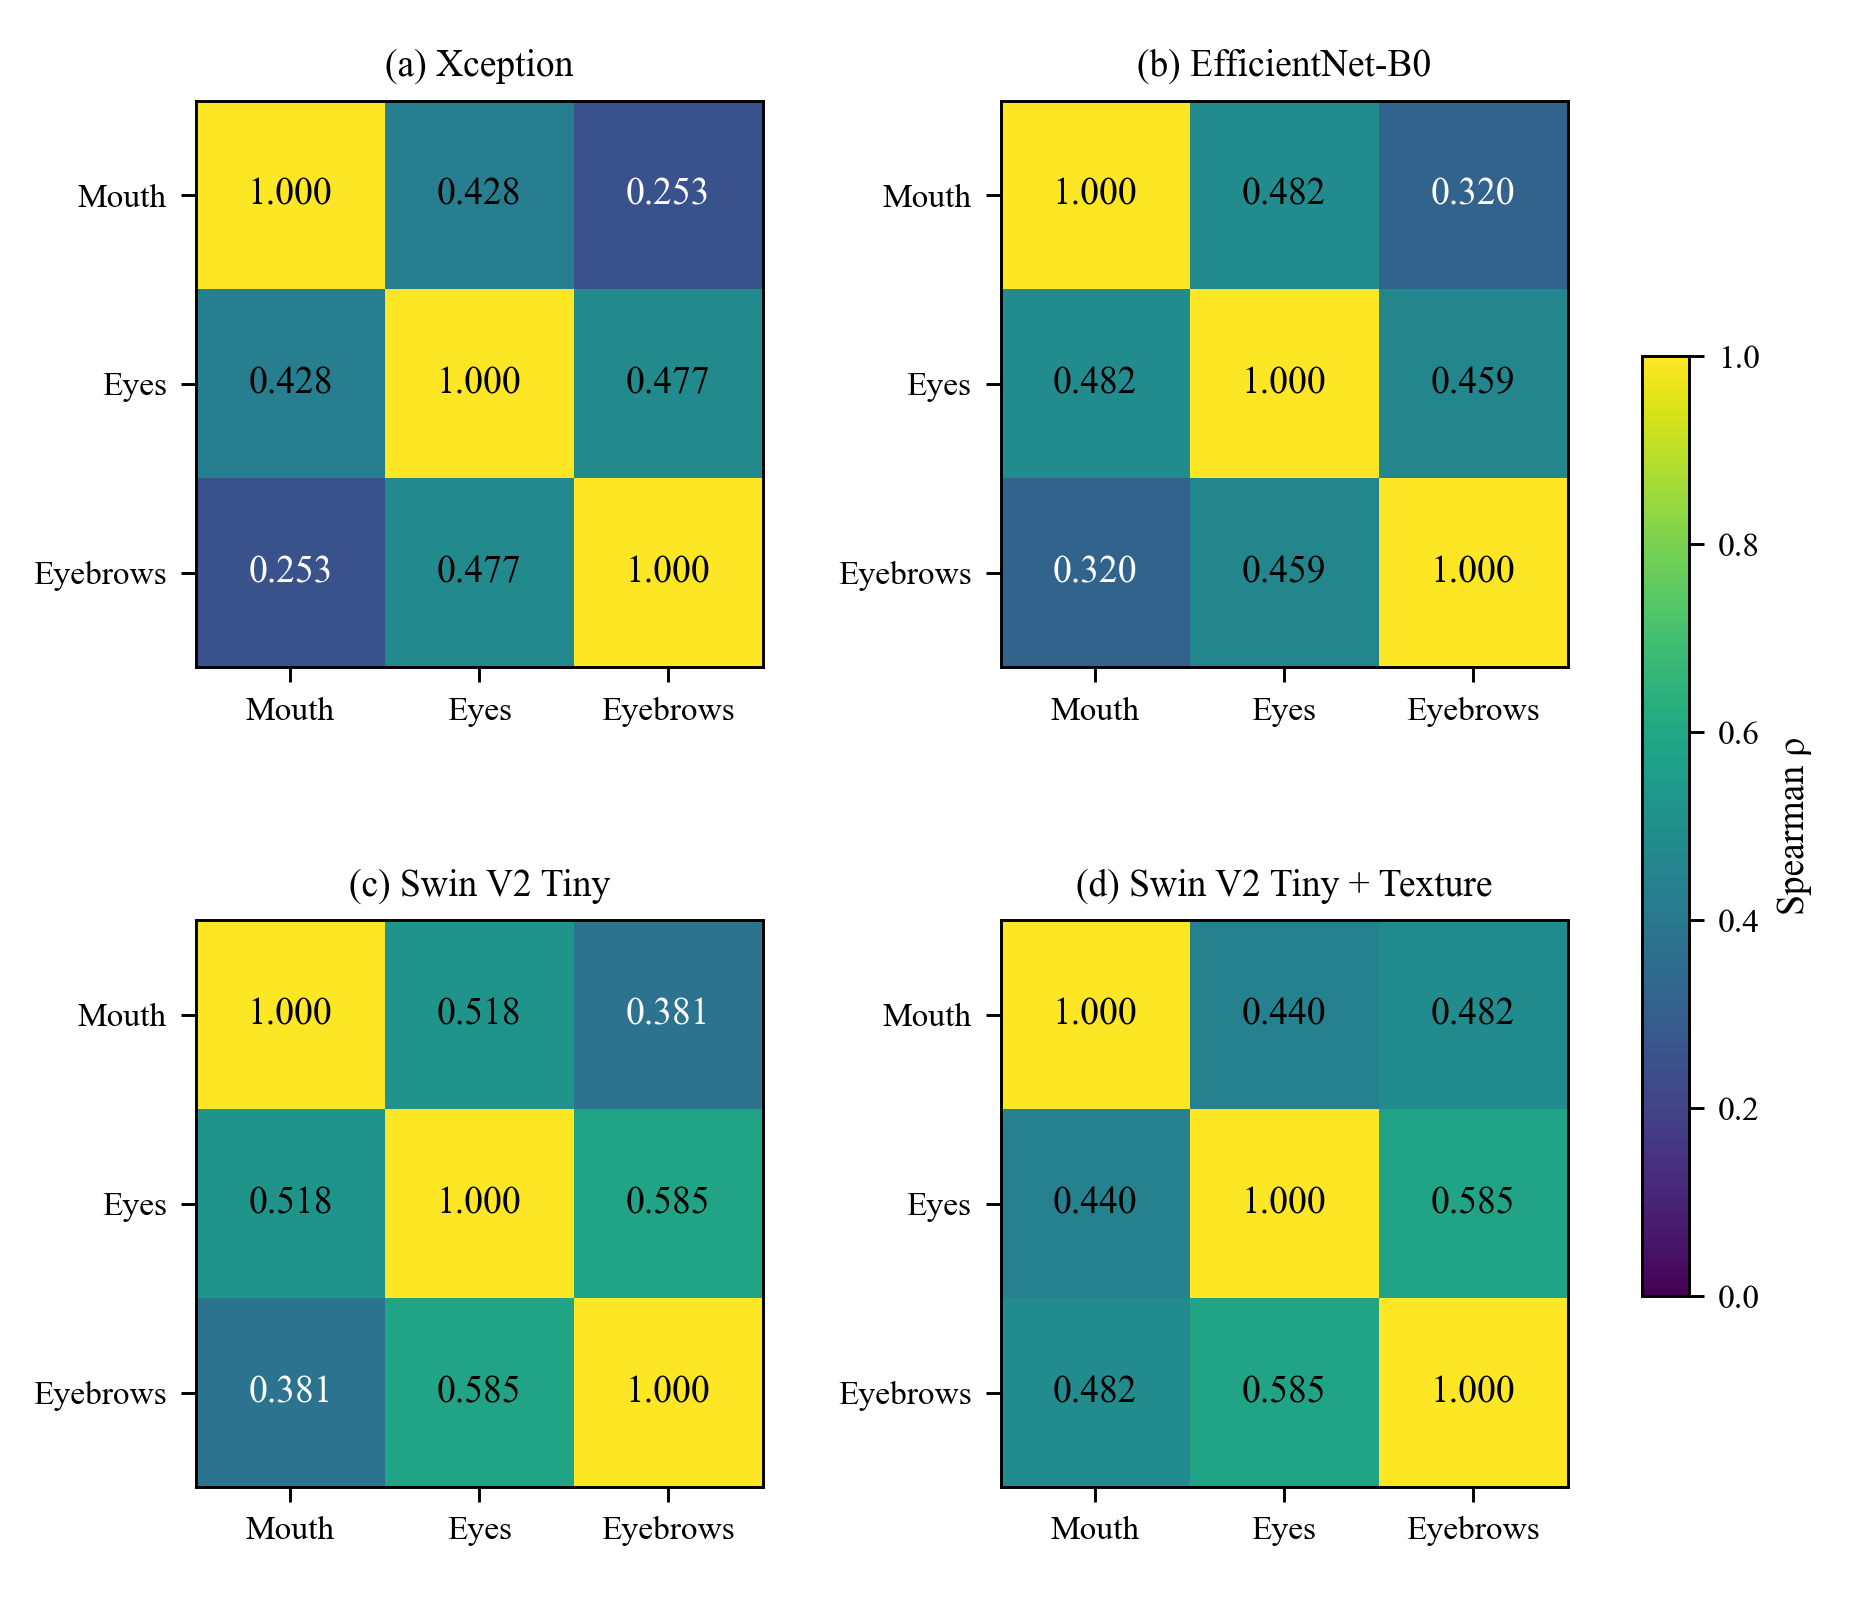
\includegraphics[width=\linewidth]{assets/correlations.png}
\caption{Spearman correlations of regional FAKE probabilities on the common cohort. (a) Xception; (b) EfficientNet-B0; (c) Swin V2 Tiny; (d) Swin V2 Tiny + Texture.}\label{fig:corr}
\end{minipage}\end{figure}

\section{Discussion}
The higher mouth ROI AUC across all four configurations suggests that mouth appearance carries discriminative information in this source pool. Lip boundaries, teeth, and intraoral textures are potential cues, but their contributions were not measured separately. The dataset-dependent regional results of Tolosana et al. \cite{tolosana} support caution against presenting the observed mouth advantage as universal anatomical superiority. Manipulation-subgroup results also show heterogeneous behavior.

LipForensics and DFT-MF use mouth motion \cite{haliassos,elhassan}, while Mirzayev and Dibeklioğlu use learnable spatiotemporal feature operations \cite{mirzayev}; these approaches examine information beyond static frames. The present mouth result cannot be attributed to motion modeling. Eye-blink analyses \cite{li,jung} similarly exploit behavioral information absent from the current static-eye experiments. Lower eyebrow performance may relate to reduced ROI availability and cropping conditions; the causal effects of data quantity and ROI quality were not isolated.

Although Swin V2 Tiny achieved the highest AUC in all three regions, the hybrid texture configuration did not exceed the base Swin model. This does not imply that all texture features are detrimental. Training settings and spatial coverage may differ, and no individual ablation analysis was conducted for LBP, GLCM, Gabor, or wavelet features. The high hybrid results reported by Shivaprakash et al. \cite{shivaprakash} were obtained with different data and protocols and should not be converted into a direct ranking against the present local-ROI results.

The fusion weighting rule combined regions according to validation performance rather than relying on a single ROI. Nevertheless, fixed weights do not model which ROI is reliable for each sample. Correcting some mouth errors while overturning some correct mouth decisions shows that complementarity does not automatically translate into an overall gain. Because no post-hoc probability calibration was performed, differences in score scales and confidence are potential contributing factors; this explanation remains a hypothesis for future testing rather than a cause established by the present results. Cross-attention-based representation fusion for localized manipulations \cite{anand} and combinations of different feature branches \cite{lei} differ from fixed averaging of ROI scores, so the findings cannot be generalized to all fusion methods.

Table~\ref{tab:literature} summarizes related studies. Their results were obtained with different datasets, ROI definitions, temporal information, and metrics; the table provides methodological context.
\begin{table}[!htbp]\centering\begin{minipage}{15.8cm}
\caption{Comparison with the methods and findings of related studies.}\label{tab:literature}
\centering \small
\begin{tabular}{>{\raggedright\arraybackslash}p{2.2cm}>{\raggedright\arraybackslash}p{3.0cm}>{\raggedright\arraybackslash}p{4.1cm}>{\raggedright\arraybackslash}p{4.1cm}}\toprule
Study & Method / scope & Reported result & Comparison limitation \\\midrule
Tolosana et al. \cite{tolosana} & Regional Xception / Capsule; UADFV, FF++, Celeb-DF, DFDC Preview. & Xception mouth AUC: 0.954 / 0.939 / 0.651 / 0.795. & Regional strength depends on the dataset. Present Xception full-test mouth AUC: 0.7662. \\
Haliassos et al. \cite{haliassos} & LipForensics; temporal mouth dynamics. & Video-level accuracy: FF++ HQ/LQ 98.8\% / 94.2\%; cross-dataset AUC: Celeb-DF v2 0.824; DFDC 0.735. & Uses different information and protocols from the present static mouth ROI. \\
Nguyen and Derakhshani \cite{nguyen} & Eyebrow biometrics; Celeb-DF and VISOB. & Approximately 0.88 AUC and 20.7\% EER. & Identity matching and static ROI classification are different tasks. \\
Soudy et al. \cite{soudy} & Eye/nose/full face; CNN/CViT and majority voting. & Approximately 96\% / 97\% accuracy for eye CNNs; 85\% accuracy in the full-face CViT experiment. & Different regions, decision fusion, and metrics prevent direct ranking against the present AUC. \\
Lei et al. \cite{lei} & Improved MTCNN-based face detection, diffusion preprocessing, geometry/texture, and decision fusion. & Multi-feature detection and adversarial-defense framework. & Differs from score fusion across three anatomical ROIs on the same cohort. \\
Shivaprakash et al. \cite{shivaprakash} & Swin V2 with LBP, GLCM, Gabor, and wavelet features. & FF++ AUC 0.9929; Celeb-DF v2 AUC 0.9962. & Under the present protocol, the hybrid ROI model did not exceed base Swin AUC. \\
Mirzayev and Dibeklioğlu \cite{mirzayev} & Learnable feature operations inspired by motion magnification networks. & Video detection examining spatiotemporal inconsistencies. & Temporal representations are outside the present static-frame experiment. \\
This study & Three ROIs, four configurations, and late fusion on 196 common samples. & Swin mouth AUC: full-test 0.8607; common cohort 0.8803. Common-cohort weighted fusion: 0.8763. & No additional AUC gain over mouth-only detection was demonstrated for equal/weighted fusion. \\
\bottomrule\end{tabular}
\par\smallskip\begin{minipage}{\linewidth}\small EER: equal error rate; HQ/LQ: high/low quality; FF++: FaceForensics++; DFDC: Deepfake Detection Challenge; CViT: convolutional vision Transformer; MTCNN: multitask cascaded convolutional neural network. External results use different protocols; no common-data reevaluation or direct superiority comparison was performed.\end{minipage}
\end{minipage}\end{table}

\subsection{Limitations}
The study is limited to one FaceForensics project pool and experimental protocol; no cross-dataset testing on an independent dataset was performed. The common fusion cohort contains only 196 samples, limiting the ability to detect small AUC differences. Lower eyebrow ROI availability restricts evaluation to a subset satisfying geometric conditions, which may not represent all source frames.

The source-folder/split check does not fully establish separation at the identity or common root-video level across all manipulations. Sample-level bootstrap does not account for video dependence, and confidence intervals may be optimistic. Because separate confidence intervals were not calculated for inter-region AUC differences, the mouth--eye--eyebrow ordering is limited to point estimates. Overlapping ROI records in the full eye/mouth tests may affect evaluation dependence. Model-specific threshold-selection rules limit accuracy/F1 comparisons, which should not be interpreted as direct evidence of architectural superiority.

Static frames do not model eye blinking or lip motion. The study includes no full-face baseline, hybrid-component ablation analysis, post-hoc calibration, or common computational-cost measurement on standardized hardware. Training budgets were not equalized, so the results do not isolate architectural superiority. Methodological work on domain generalization \cite{karimi} supports the need for separate evaluation on external data.

\section{Conclusion and future work}
Under the present protocol, the mouth ROI yielded the highest regional ROC-AUC point estimate for all four model configurations. Swin V2 Tiny achieved the highest AUC in all three ROIs, while the hybrid texture configuration did not exceed the base Swin model. On the common test cohort, validation-weighted fusion yielded higher AUC than equal fusion but did not surpass mouth-only performance in any configuration. Bootstrap confidence intervals for the differences included zero, so no additional fusion gain was demonstrated and the observed decreases were not statistically distinguishable. The mouth ROI therefore emerges as a strong single-region option within the present data and protocol.

Future work may focus on independent datasets, improved eye/eyebrow ROI quality, regional score calibration, and adaptive fusion based on sample or ROI reliability. Preserving source-video identifiers would enable video-cluster bootstrap; temporal models, full-face comparisons, and hybrid-component analyses could also be added. 

\section*{Data and code availability}
Raw videos and images are not redistributed; access is subject to the terms of use and licenses of the respective data sources. Code repository: \url{https://github.com/aiscdeepfake/AISC-DeepFake-Detection}. The conditions governing raw data sources apply separately from code access.
\FloatBarrier
\begin{thebibliography}{99}
\bibitem{rossler} Rössler A, Cozzolino D, Verdoliva L, Riess C, Thies J et al. FaceForensics++: Learning to detect manipulated facial images. In: Proceedings of the IEEE/CVF International Conference on Computer Vision; Seoul, South Korea; 2019. pp. 1--11. \url{https://doi.org/10.1109/iccv.2019.00009}
\bibitem{tolosana} Tolosana R, Romero-Tapiador S, Fierrez J, Vera-Rodriguez R. DeepFakes evolution: Analysis of facial regions and fake detection performance. In: Pattern Recognition. ICPR International Workshops and Challenges. LNCS 12665; 2021. pp. 442--456. \url{https://doi.org/10.1007/978-3-030-68821-9_38}
\bibitem{zhao} Zhao H, Zhou W, Chen D, Wei T, Zhang W et al. Multi-attentional deepfake detection. In: Proceedings of the IEEE/CVF Conference on Computer Vision and Pattern Recognition; Online; 2021. pp. 2185--2194. \url{https://doi.org/10.1109/cvpr46437.2021.00222}
\bibitem{chollet} Chollet F. Xception: Deep learning with depthwise separable convolutions. In: Proceedings of the IEEE Conference on Computer Vision and Pattern Recognition; Honolulu, HI, USA; 2017. pp. 1251--1258. \url{https://doi.org/10.1109/cvpr.2017.195}
\bibitem{tan} Tan M, Le Q. EfficientNet: Rethinking model scaling for convolutional neural networks. In: Proceedings of the 36th International Conference on Machine Learning; Long Beach, CA, USA; 2019. PMLR 97, pp. 6105--6114.
\bibitem{swin} Liu Z, Hu H, Lin Y, Yao Z, Xie Z et al. Swin Transformer V2: Scaling up capacity and resolution. In: Proceedings of the IEEE/CVF Conference on Computer Vision and Pattern Recognition; New Orleans, LA, USA; 2022. pp. 12009--12019. \url{https://doi.org/10.1109/cvpr52688.2022.01170}
\bibitem{li} Li Y, Chang MC, Lyu S. In ictu oculi: Exposing AI created fake videos by detecting eye blinking. In: IEEE International Workshop on Information Forensics and Security; Hong Kong, China; 2018. pp. 1--7. \url{https://doi.org/10.1109/wifs.2018.8630787}
\bibitem{jung} Jung T, Kim S, Kim K. DeepVision: Deepfakes detection using human eye blinking pattern. IEEE Access 2020; 8: 83144--83154. \url{https://doi.org/10.1109/ACCESS.2020.2988660}
\bibitem{haliassos} Haliassos A, Vougioukas K, Petridis S, Pantic M. Lips don’t lie: A generalisable and robust approach to face forgery detection. In: Proceedings of the IEEE/CVF Conference on Computer Vision and Pattern Recognition; Online; 2021. pp. 5039--5049. \url{https://doi.org/10.1109/cvpr46437.2021.00500}
\bibitem{elhassan} Elhassan A, Al-Fawa’reh M, Jafar MT, Ababneh M, Jafar ST. DFT-MF: Enhanced deepfake detection using mouth movement and transfer learning. SoftwareX 2022; 19: 101115. \url{https://doi.org/10.1016/j.softx.2022.101115}
\bibitem{nguyen} Nguyen HM, Derakhshani R. Eyebrow recognition for identifying deepfake videos. In: International Conference of the Biometrics Special Interest Group; Online; 2020. pp. 199--206.
\bibitem{soudy} Soudy AH, Sayed O, Tag-Elser H, Ragab R, Mohsen S et al. Deepfake detection using convolutional vision transformers and convolutional neural networks. Neural Computing and Applications 2024; 36 (31): 19759--19775. \url{https://doi.org/10.1007/s00521-024-10181-7}
\bibitem{mirzayev} Mirzayev A, Dibeklioğlu H. Motion magnification-inspired feature manipulation for deepfake detection. Turkish Journal of Electrical Engineering and Computer Sciences 2024; 32 (1): 166--182. \url{https://doi.org/10.55730/1300-0632.4061}
\bibitem{anand} Anand T, Sankar S, Nair P. Detecting localized deepfake manipulations using action unit-guided video representations. In: Proceedings of the IEEE/CVF Conference on Computer Vision and Pattern Recognition Workshops; Nashville, TN, USA; 2025. pp. 4380--4390. \url{https://doi.org/10.1109/cvprw67362.2025.00419}
\bibitem{lei} Lei S, Song J, Feng F, Yan Z, Wang A. Deepfake face detection and adversarial attack defense method based on multi-feature decision fusion. Applied Sciences 2025; 15 (12): 6588. \url{https://doi.org/10.3390/app15126588}
\bibitem{shivaprakash} Shivaprakash SJ, Chauhan A, Sabireen H, Abdul Quadir Md. Hybrid facial deepfake detection framework using Swin V2 vision transformers and multi-scale textural descriptors. Signal, Image and Video Processing 2026; 20: 233. \url{https://doi.org/10.1007/s11760-026-05279-5}
\bibitem{karimi} Karimi S, Dibeklioğlu H. Uncovering and mitigating spurious features in domain generalization. Turkish Journal of Electrical Engineering and Computer Sciences 2024; 32 (2): 320--337. \url{https://doi.org/10.55730/1300-0632.4071}
\end{thebibliography}
\end{document}
